\documentclass{beamer}
\usepackage[utf8]{inputenc}
\usepackage{graphicx, epsfig}
\usepackage{amsmath,mathrsfs,amsfonts,amssymb}
%\usepackage{subfig}
\usepackage{floatflt}
\usepackage{epic,ecltree}
\usepackage{mathtext}
\usepackage{fancybox}
\usepackage{fancyhdr}
\usepackage{multirow}
\usepackage{enumerate}
\usepackage{epstopdf}
\usepackage{multicol}
\usepackage{algorithm}
\usepackage[noend]{algorithmic}
\def\algorithmicrequire{\textbf{Input:}}
\def\algorithmicensure{\textbf{Output:}}
\usetheme{default}%{Singapore}%{Warsaw}%{Warsaw}%{Darmstadt}
\usecolortheme{default}
\setbeamertemplate{footline}[page number]{}
\setbeamerfont{title}{size=\Huge}

\newcommand{\bt}{\mathbf{t}} 
\newcommand{\bu}{\mathbf{u}} 
\newcommand{\bw}{\mathbf{w}} 
\newcommand{\bx}{\mathbf{x}} 
\newcommand{\bz}{\mathbf{z}} 
\newcommand{\by}{\mathbf{y}} 

\newcommand{\bI}{\mathbf{I}} 
\newcommand{\bT}{\mathbf{T}} 
\newcommand{\bU}{\mathbf{U}} 
\newcommand{\bX}{\mathbf{X}} 
\newcommand{\bY}{\mathbf{Y}} 
\newcommand{\bZ}{\mathbf{Z}} 

\newcommand{\bepsilon}{\boldsymbol{\epsilon}}
\newcommand{\bmu}{\boldsymbol{\mu}}
\newcommand{\blambda}{\boldsymbol{\lambda}}
\newcommand{\bsigma}{\boldsymbol{\sigma}}

\newcommand{\btheta}{\boldsymbol{\theta}} 
\newcommand{\bphi}{\boldsymbol{\phi}} 

\DeclareMathOperator*{\argmin}{arg\,min}
\DeclareMathOperator*{\argmax}{arg\,max}

%\definecolor{beamer@blendedblue}{RGB}{15,120,80}
%----------------------------------------------------------------------------------------------------------
\title[\hbox to 56mm{Deep Generative Models  \hfill\insertframenumber\,/\,\inserttotalframenumber}]
{Deep Generative Models \\ Lecture 5}
\author[Roman Isachenko]{\\Roman Isachenko}
\institute[MIPT]{Moscow Institute of Physics and Technology \\
}
\date{2020}
%--------------------------------------------------------------------------------
\begin{document}
%--------------------------------------------------------------------------------
\begin{frame}
%\thispagestyle{empty}
\titlepage
\end{frame}
%=======
\begin{frame}{Glow, 2018}
	\begin{figure}
		\centering
		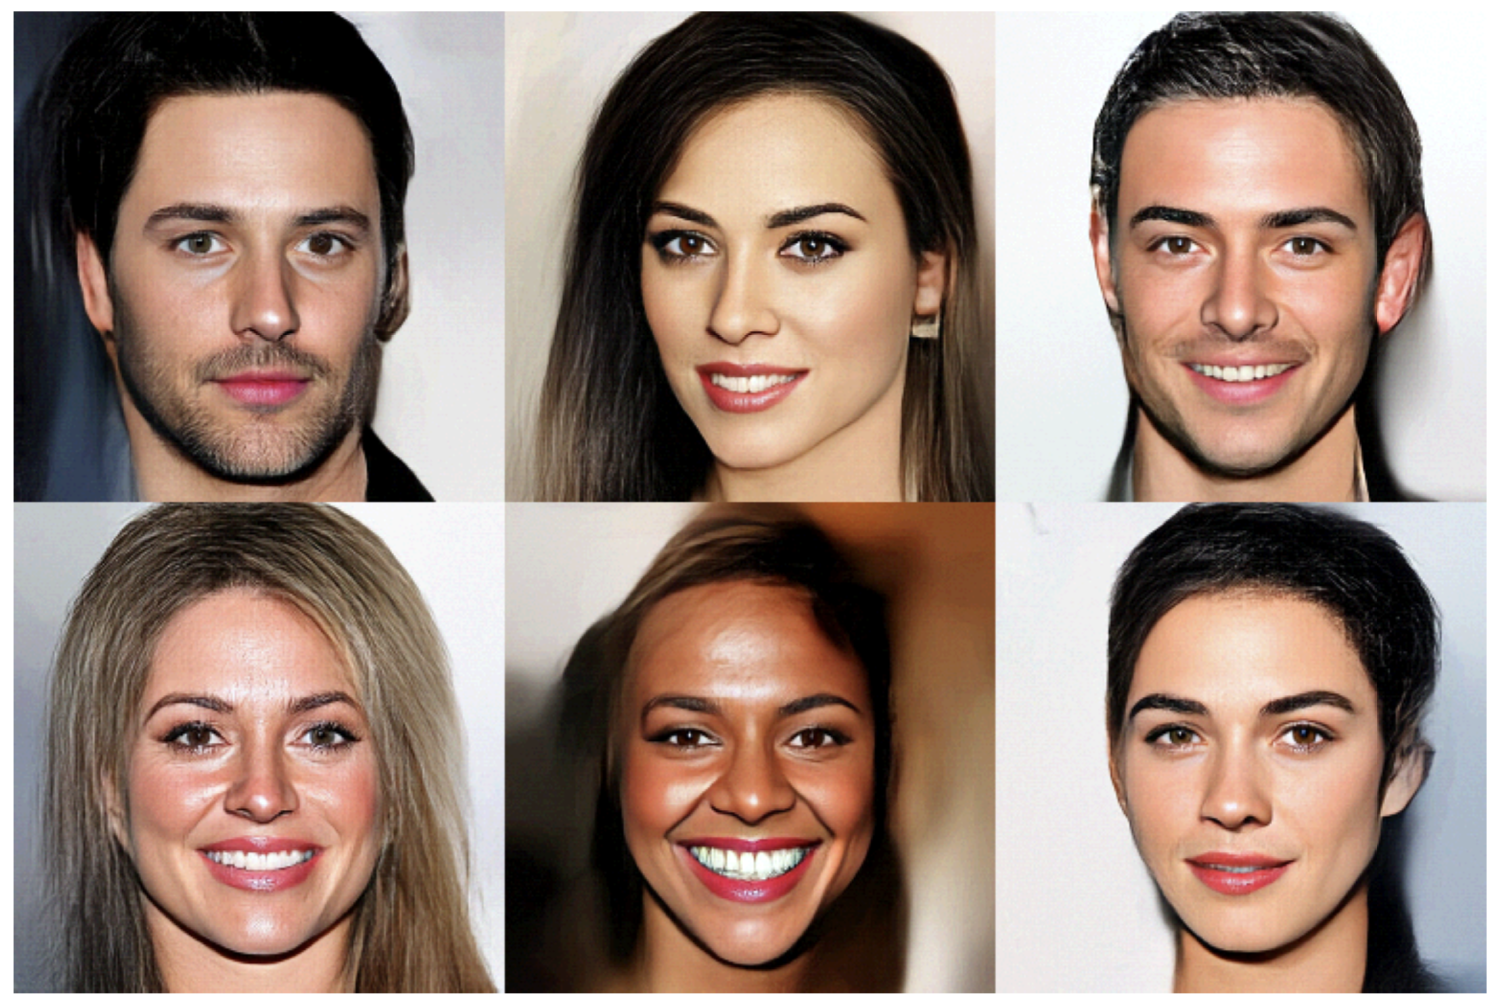
\includegraphics[width=\linewidth]{figs/glow_faces.png}
	\end{figure}
	\vfill
	\hrule\medskip
	{\scriptsize \href{https://arxiv.org/pdf/1807.03039.pdf}{https://arxiv.org/pdf/1807.03039.pdf}} 
\end{frame}
%=======
\begin{frame}{Glow, 2018}
	\begin{block}{Model architecture}
		\begin{figure}
			\centering
			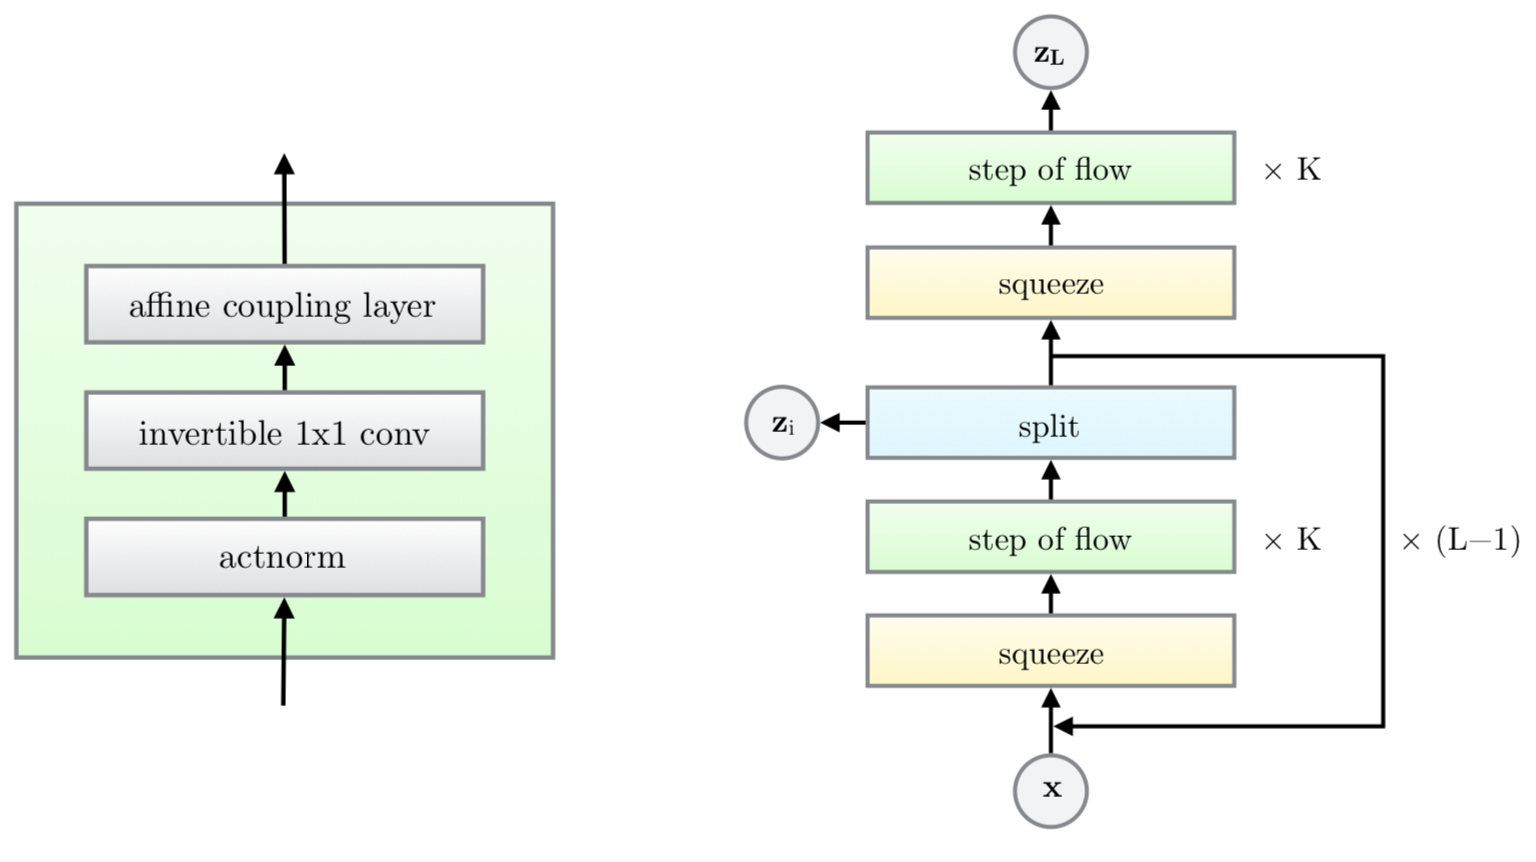
\includegraphics[width=\linewidth]{figs/glow_block.png}
		\end{figure}
	\end{block}
	\vfill
	\hrule\medskip
	{\scriptsize \href{https://arxiv.org/pdf/1807.03039.pdf}{https://arxiv.org/pdf/1807.03039.pdf}}   
\end{frame}
%=======
\begin{frame}{Glow, 2018}
	
	\begin{block}{NICE}
		\vspace{-0.2cm}
		\begin{equation*}
			\begin{cases} \bz_1 = \bx_1; \\ \bz_2 = \bx_2 + \mathcal{F}(\bx_1, \btheta);\end{cases}  \quad \Leftrightarrow \quad 
			\begin{cases} \bx_1 = \bz_1; \\ \bx_2 = \bz_2 - \mathcal{F}(\bz_1, \btheta).\end{cases} 
		\end{equation*}
		\vspace{-0.2cm}
	\end{block}
	
	First step is a \textbf{split} operator which decouples variable into 2 subparts (usualy channel-wise).
	The order of decoupling should be manually changed between layers.
	
	Could we use more general operator?
	
	Let use rotation matrix via 1x1 invertible convolution.
	
	$\mathbf{W} \in \mathbb{R}^{c \times c}$ - kernel of 1x1 convolution with $c$ input and output channels.
	
	The cost of computing or differentiating $\det (\mathbf{W})$ is $O(c^3)$.
	
	\vfill
	\hrule\medskip
	{\scriptsize \href{https://arxiv.org/pdf/1807.03039.pdf}{https://arxiv.org/pdf/1807.03039.pdf}}    
\end{frame}
%=======
\begin{frame}{Glow, 2018}
	\begin{figure}
		\centering
		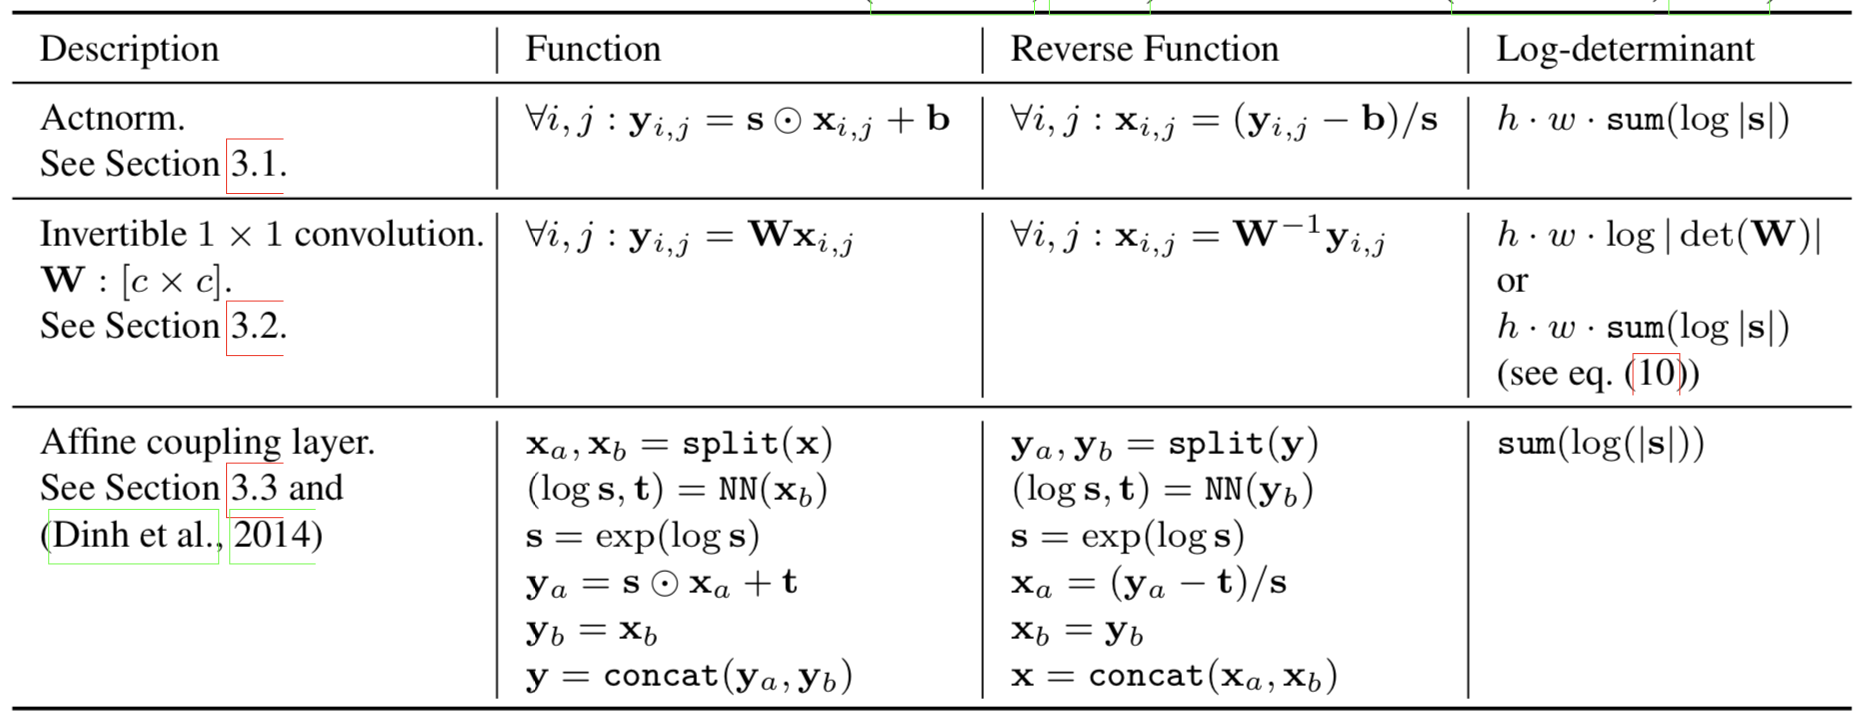
\includegraphics[width=\linewidth]{figs/glow_ops.png}
	\end{figure}
	\vfill
	\hrule\medskip
	{\scriptsize \href{https://arxiv.org/pdf/1807.03039.pdf}{https://arxiv.org/pdf/1807.03039.pdf}}    
\end{frame}
%=======
\begin{frame}{Glow, 2018}
	\begin{block}{Invertible 1x1 conv}
		Cost to compute $\det (\mathbf{W})$ is $O(c^3)$. 
		LU-decomposition reduces the cost to $O(c)$:
		\[
		\mathbf{W} = \mathbf{P}\mathbf{L}(\mathbf{U} + \text{diag}(\mathbf{s})),
		\]
		where $\mathbf{P}$ is a permutation matrix, $\mathbf{L}$ is a lower triangular matrix with ones on the diagonal, $\mathbf{U}$ is an
		upper triangular matrix with zeros on the diagonal, and $\mathbf{s}$ is a vector.
	\end{block}
	\begin{figure}
		\centering
		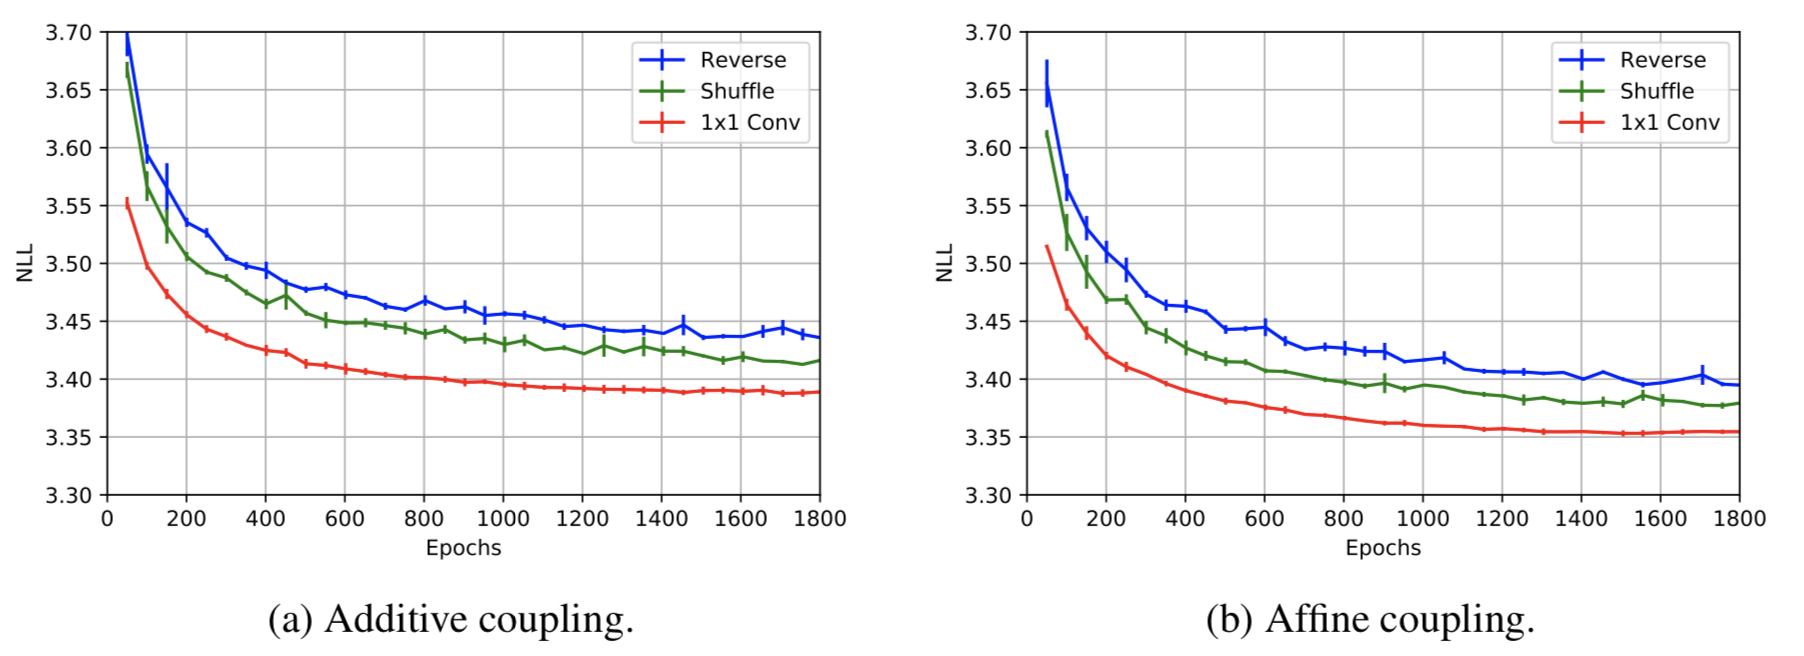
\includegraphics[width=\linewidth]{figs/glow_1x1_conv.png}
	\end{figure}
	\vfill
	\hrule\medskip
	{\scriptsize \href{https://arxiv.org/pdf/1807.03039.pdf}{https://arxiv.org/pdf/1807.03039.pdf}}    
\end{frame}
%=======
\begin{frame}{Glow, 2018}
	\begin{block}{Face interpolation}
		\begin{figure}
			\centering
			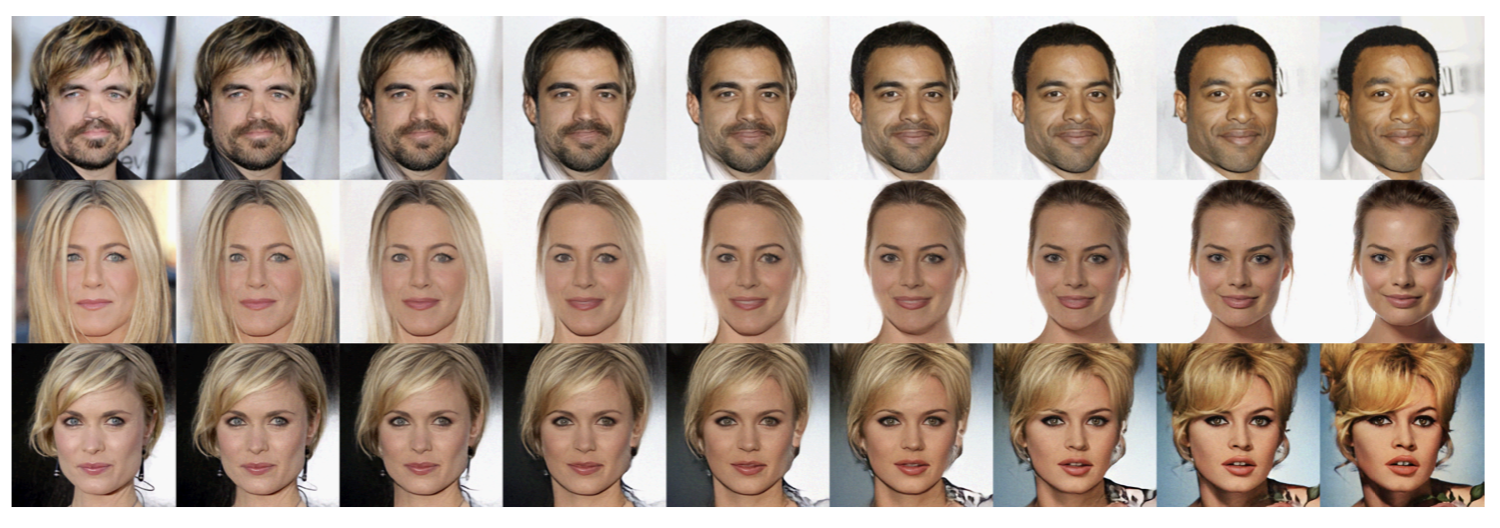
\includegraphics[width=\linewidth]{figs/glow_interpolation.png}
		\end{figure}
	\end{block}
	\vfill
	\hrule\medskip
	{\scriptsize \href{https://arxiv.org/pdf/1807.03039.pdf}{https://arxiv.org/pdf/1807.03039.pdf}}   
\end{frame}
%=======
\begin{frame}{Glow, 2018}
	\begin{block}{Face attributes manipulation}
		\begin{figure}
			\centering
			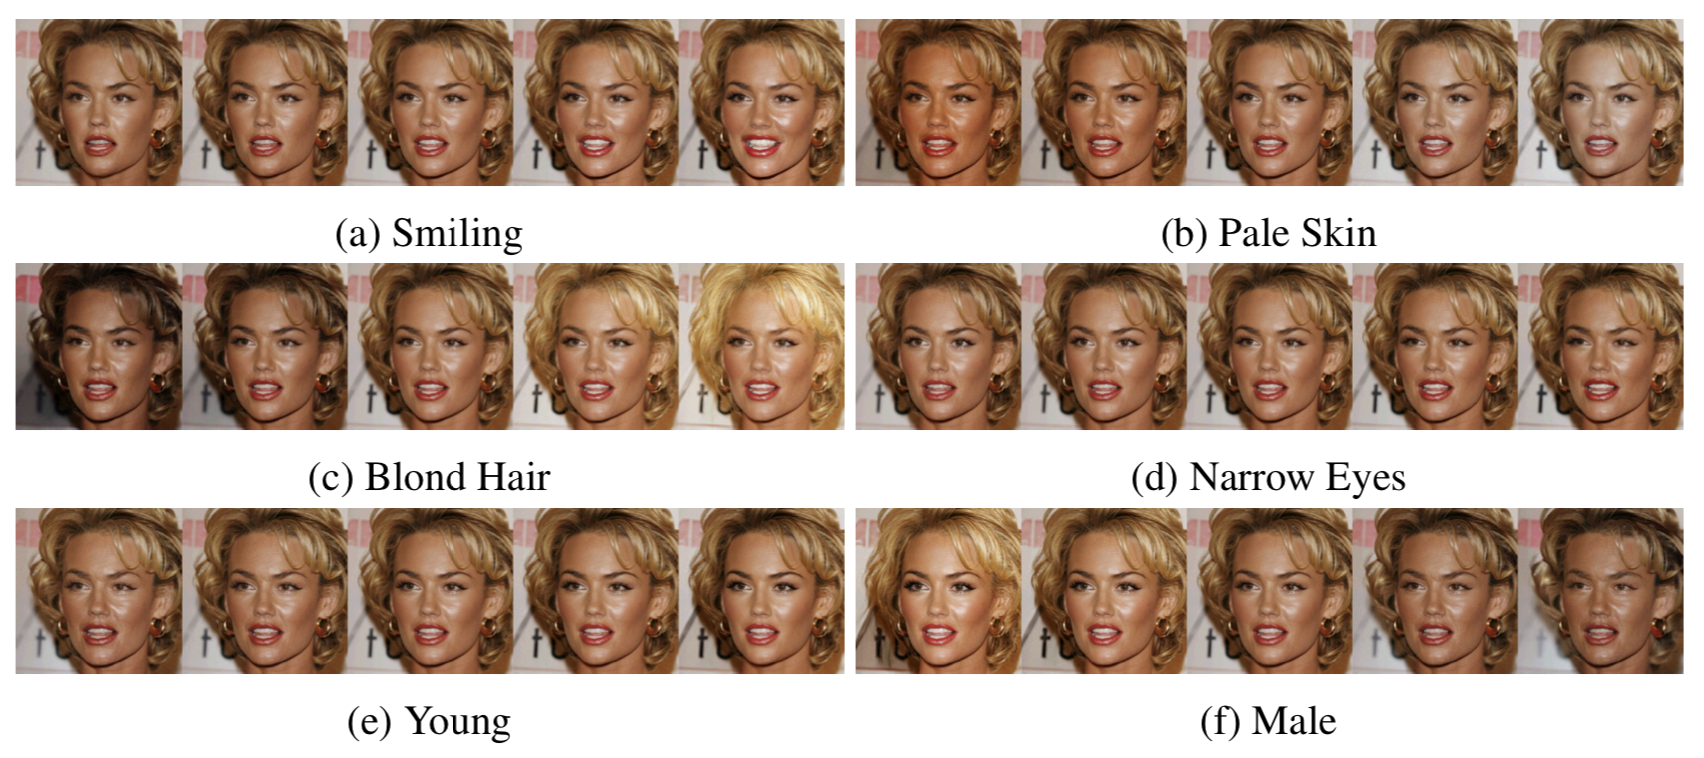
\includegraphics[width=\linewidth]{figs/glow_attributes.png}
		\end{figure}
	\end{block}
	\vfill
	\hrule\medskip
	{\scriptsize \href{https://arxiv.org/pdf/1807.03039.pdf}{https://arxiv.org/pdf/1807.03039.pdf}}   
\end{frame}
\begin{frame}{Summary}
	\begin{itemize}
		\item Flows are generative models with tractable likelihood and latent representation.
		\item Flows transform simple distributions to the complex one via sequence of invertible transformations.
		\item The goal is to achieve tractable Jacobian for efficient learning and density estimation.
	\end{itemize}
\end{frame}
%=======
\begin{frame}{Dequantization}
	\begin{itemize}
		\item Images are discrete data (pixels lies in the [0, 255] integer domain). 
		\item Flow is a continuous model.
	\end{itemize}
	Fitting a continuous density model to discrete data, produces a degenerate solution with all probability mass on discrete values. \\
	How to convert discrete data distribution to the continuous one?
	
	\begin{minipage}[t]{0.5\columnwidth}
		\begin{block}{Uniform dequantization}
			\[
			\by = \bx + \bu, \quad \bu \sim U[0, 1]
			\]
		\end{block}
	\end{minipage}%
	\begin{minipage}[t]{0.5\columnwidth}
		\begin{figure}
			\centering
			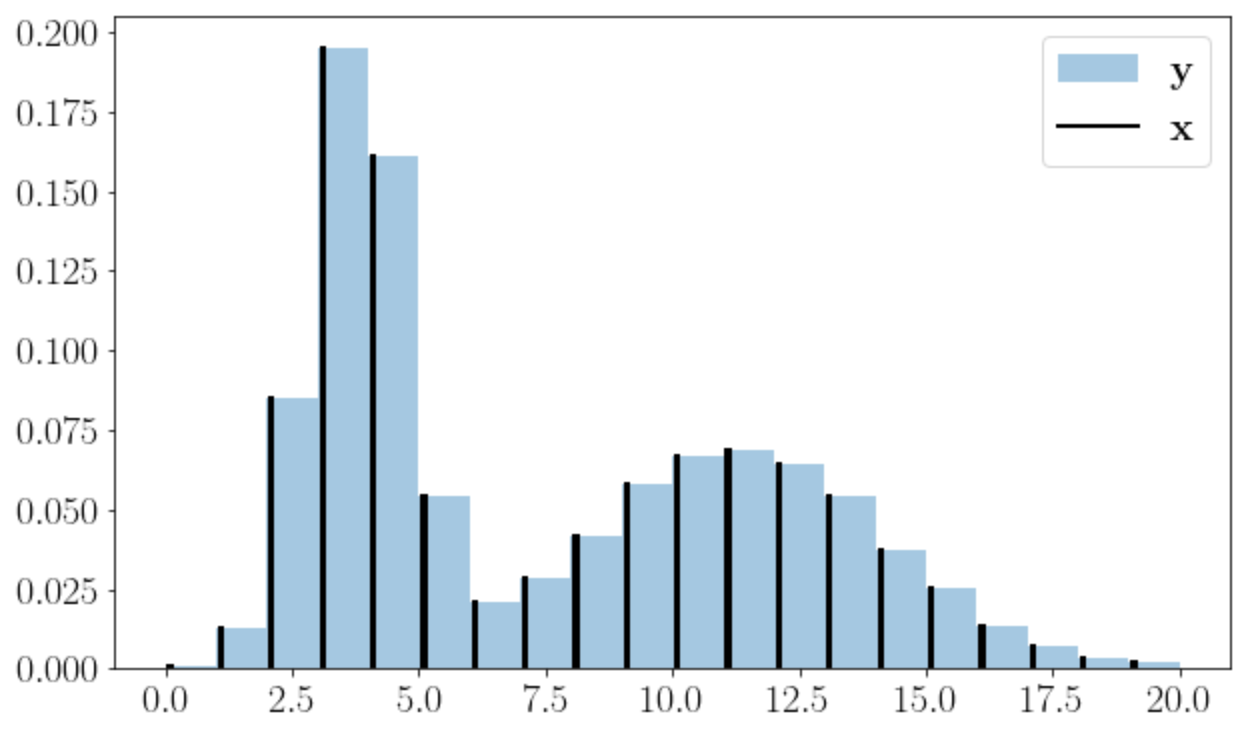
\includegraphics[width=1.0\linewidth]{figs/uniform_dequantization.png}
		\end{figure}
	\end{minipage}
\end{frame}
%=======
\begin{frame}{Uniform dequantization}
	\begin{block}{Statement}
		Fitting continious model $p(\by | \btheta)$ on uniformly dequantized data $\by = \bx + \bu, \, \bu \sim U[0, 1]$ is equivalent to maximization of a lower bound on the log-likelihood for a discrete model:
		\[
		P(\bx | \btheta) = \int_{U[0, 1]} p(\bx + \bu | \btheta) d \bu
		\]
		\vspace{-0.2cm} \\
		Thus, maximizing the log-likelihood of the continuous model on $\by$ cannot lead to the collapsing onto the discrete data (objective is bounded above by the log-likelihood of a discrete model).
	\end{block}
	\begin{block}{Proof}
		\vspace{-1cm}
		\begin{multline*}
			\log p(\bY | \btheta) = \sum_{i = 1}^n \log p(\by_i | \btheta) = \sum_{i = 1}^n \int_{U[0, 1]} \log p(\bx_i + \bu | \btheta) d \bu \\ \leq \sum_{i = 1}^n \log \int_{U[0, 1]} p(\bx_i + \bu | \btheta) d \bu = \sum_{i=1}^n \log P(\bx_i | \btheta).
		\end{multline*}
	\end{block}
\end{frame}
%=======
\begin{frame}{Variational dequantization}
	\begin{minipage}[t]{0.5\columnwidth}
			\begin{figure}
				\centering
				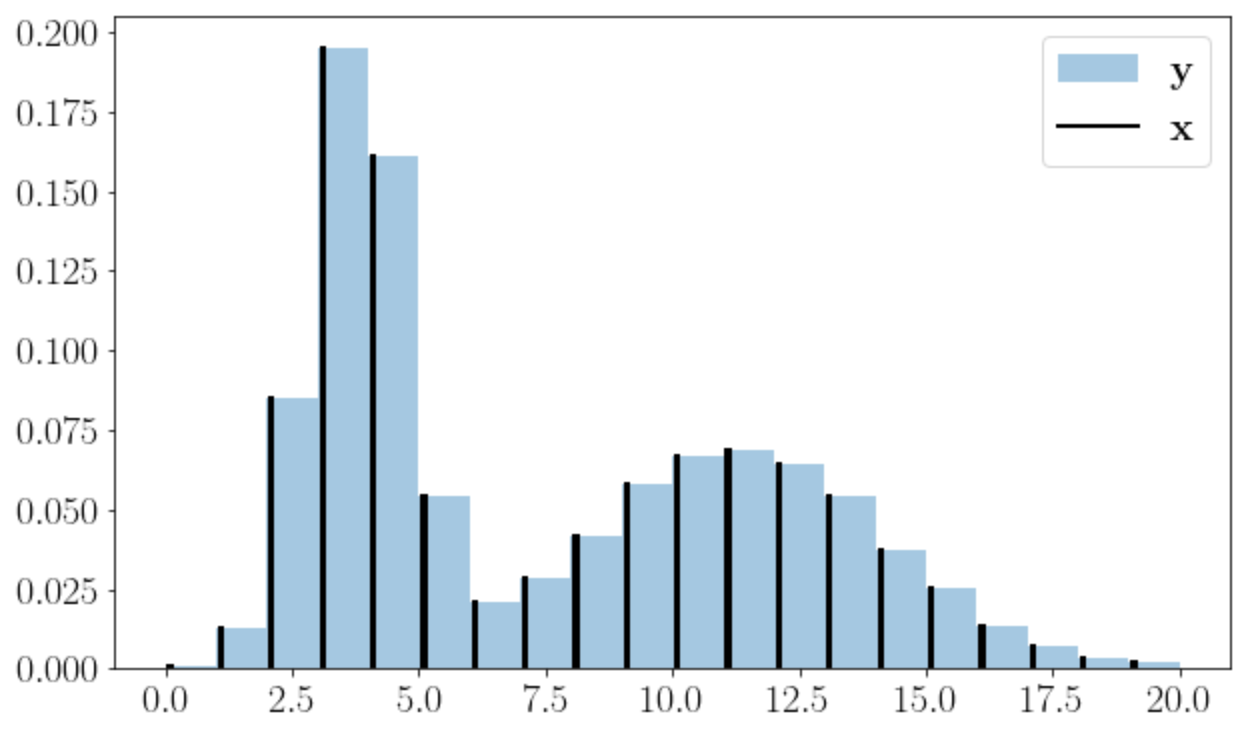
\includegraphics[width=1.0\linewidth]{figs/uniform_dequantization.png}
			\end{figure}
	\end{minipage}%
	\begin{minipage}[t]{0.5\columnwidth}
		\begin{figure}
			\centering
			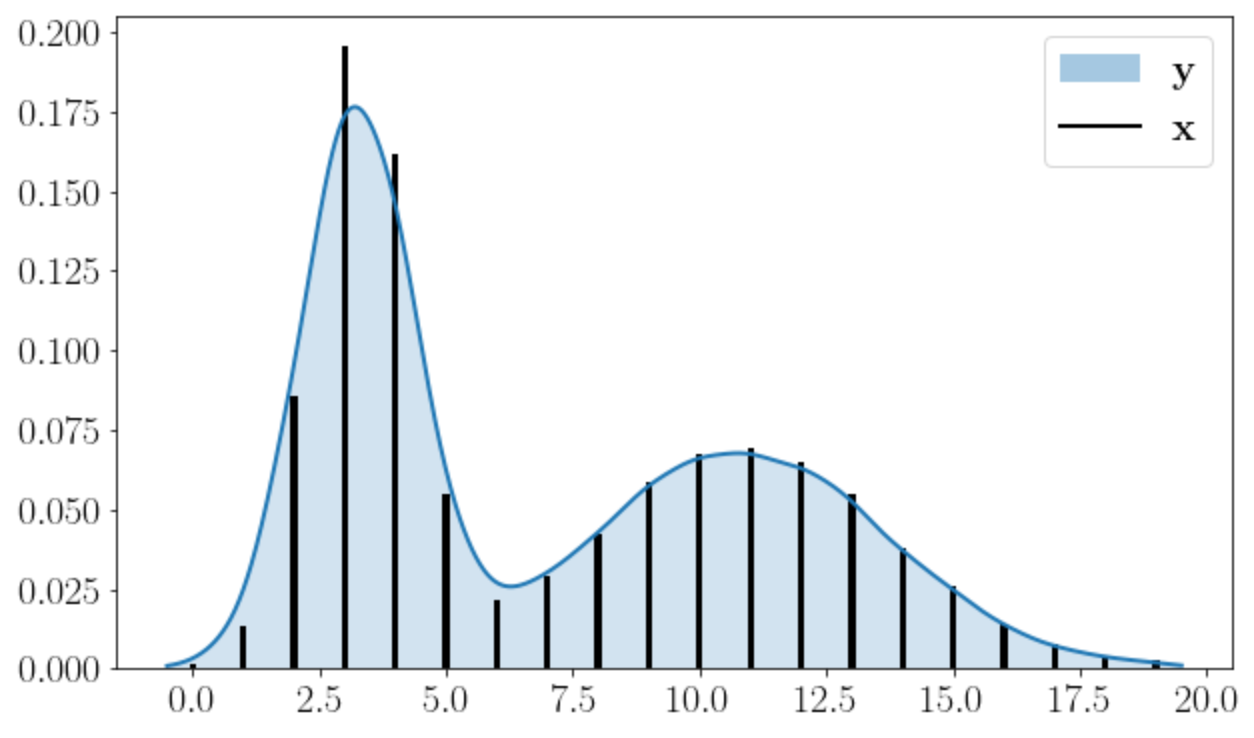
\includegraphics[width=1.0\linewidth]{figs/variational_dequantization.png}
		\end{figure}
	\end{minipage}
	\begin{itemize}
		\item $p(\by | \btheta)$ assign unifrom density to unit hypercubes $\bx + U[0, 1]$ (left fig).
		\item Neural network density models is a smooth function approximator (right fig).
		\item Smooth dequantization is more natural.
	\end{itemize}
	How to make the smooth dequantization? \\
\end{frame}
%=======
\begin{frame}{Flow++}
	\begin{block}{Variational dequantization}
		Introduce variational dequantization noise distribution $q(\bu | \bx)$ and treat it as an approximate posterior. 
	\end{block}
	\begin{block}{Variational lower bound}
		\begin{multline*}
			\log P(\bX | \btheta) = \sum_{i=1}^n \log P(\bx_i | \btheta) = \sum_{i=1}^n \left[ \log \int q(\bu | \bx) \frac{p(\bx + \bu | \btheta)}{q(\bu | \bx)} d \bu \right] \geq \\ 
			\geq\sum_{i=1}^n \left[  \int q(\bu | \bx) \log \frac{p(\bx + \bu | \btheta)}{q(\bu | \bx)} d \bu \right] = \\ = \int q(\bU | \bX) \log \frac{p(\bX + \bU | \btheta)}{q(\bU | \bX)} d \bU = \mathcal{L}(q, \btheta).
		\end{multline*}
	\end{block}
	\hrule\medskip
	{\scriptsize \href{https://arxiv.org/pdf/1902.00275.pdf}{https://arxiv.org/pdf/1902.00275.pdf}}
\end{frame}
%=======
\begin{frame}{Flow++}
	\begin{block}{Variational lower bound}
		\[
		\mathcal{L}(q, \btheta) = \int q(\bU | \bX) \log \frac{p(\bX + \bU | \btheta)}{q(\bU | \bX)} d \bU.
		\]
	\end{block}
	Let $\bu = h(\bepsilon)$ is a flow model with base distribution $\bepsilon \sim p(\bepsilon) = \mathcal{N}(0, \mathbf{I})$:
	\[
		q(\bu | \bx) = p(h^{-1}(\bu)) \cdot \left| \det \frac{\partial h^{-1}(\bu)}{\partial \bu}\right|.
	\]
	Then
	\[
		\log P(\bX | \btheta) \geq \sum_{i=1}^n \int \log \left( \frac{p(\bx + h(\bepsilon))}{p(\bepsilon) \cdot \left| \det \frac{\partial h(\bepsilon)}{\partial \bepsilon}\right|^{-1}} \right) d\bepsilon.
	\]
	\hrule\medskip
	{\scriptsize \href{https://arxiv.org/pdf/1902.00275.pdf}{https://arxiv.org/pdf/1902.00275.pdf}}
\end{frame}
%=======
\begin{frame}{Flow++}
	\[
		\log P(\bX | \btheta) \geq \sum_{i=1}^n \int \log \left( \frac{p(\bx + h(\bepsilon))}{p(\bepsilon) \cdot \left| \det \frac{\partial h(\bepsilon)}{\partial \bepsilon}\right|^{-1}} \right) d\bepsilon.
	\]
	If $p(\bx + \bu | \btheta)$ is also a flow model, it is straightforward to calculate stochastic gradient of this ELBO.
	
	\textbf{Note:} Uniform dequantization is a special case of variational dequantization ($q(\bu | \bx) = U[0, 1]$).
	The gap between $\log P(\bX | \btheta)$ and the derived ELBO is 
	\[
		KL(q(\bU | \bX) || p(\bU | \bX)).
	\]
	In the case of uniform dequantization the model unnaturally places uniform density over each hypercube $\bx + U[0, 1]$ due to inexpressive distribution $q$.
	\vfill
	\hrule\medskip
	{\scriptsize \href{https://arxiv.org/pdf/1902.00275.pdf}{https://arxiv.org/pdf/1902.00275.pdf}}
\end{frame}
%=======
\begin{frame}{Flow++}
	\begin{figure}
		\centering
		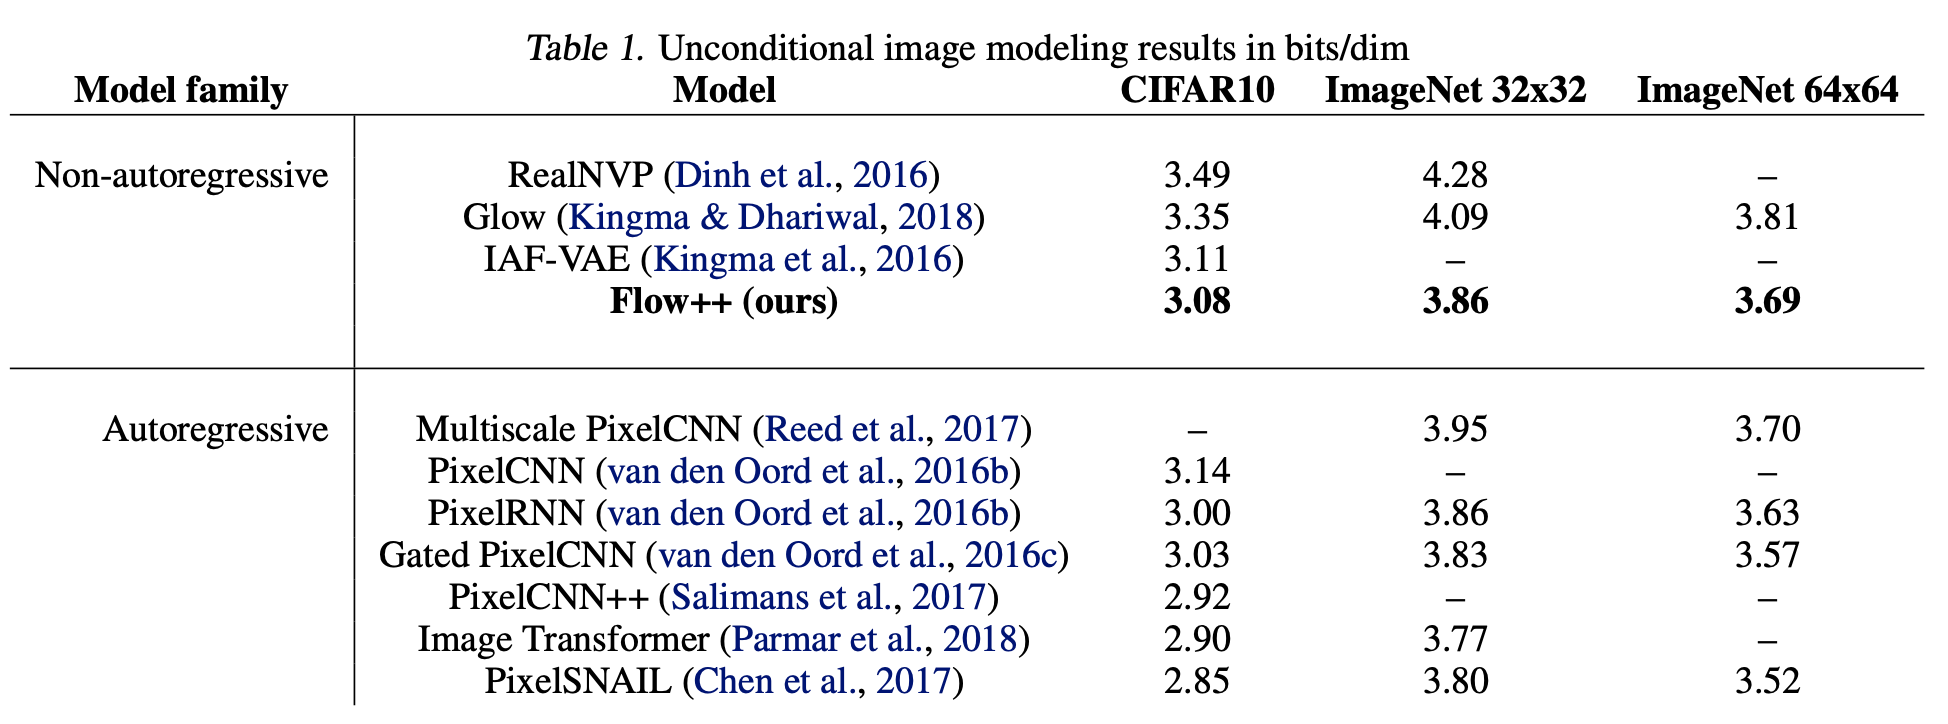
\includegraphics[width=0.7\linewidth]{figs/flow++1.png}
	\end{figure}
	\vspace{-0.1cm}
	\begin{figure}
		\centering
		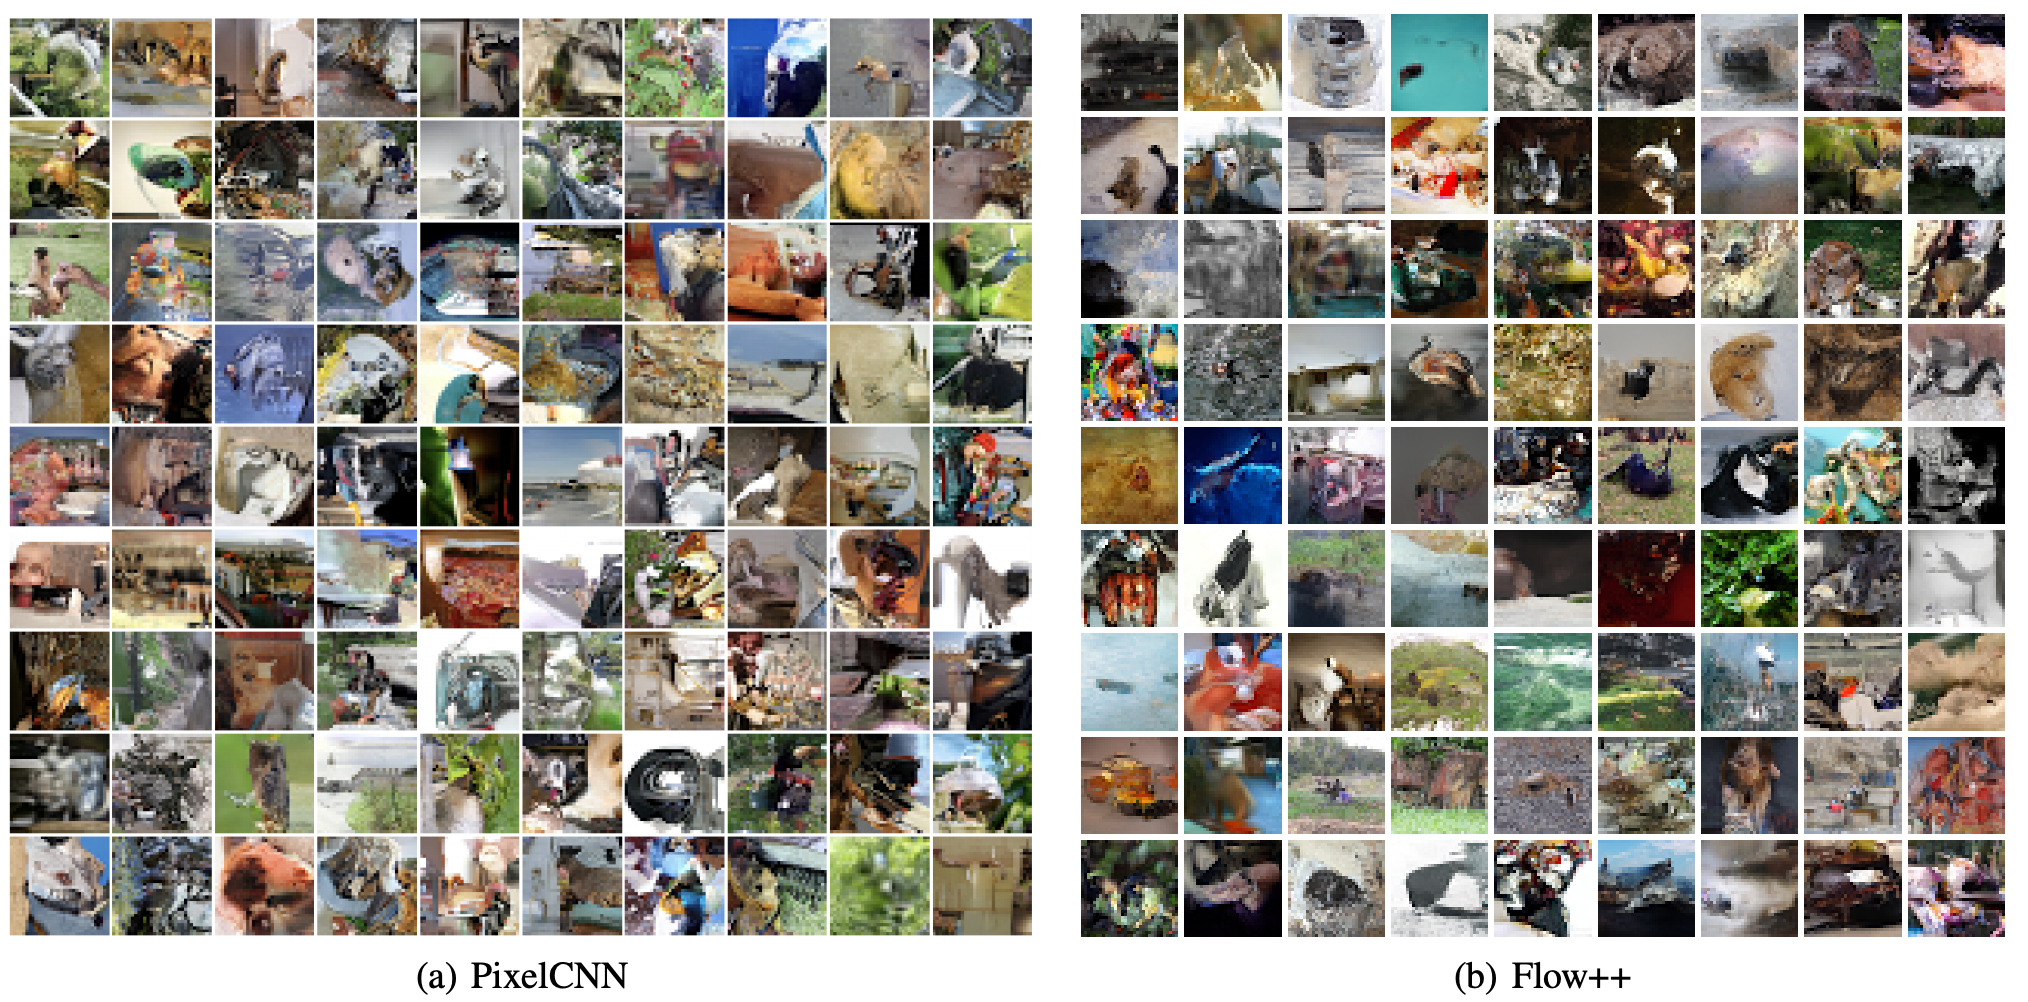
\includegraphics[width=0.8\linewidth]{figs/flow++2.png}
	\end{figure}
	\vfill
	\hrule\medskip
	{\scriptsize \href{https://arxiv.org/pdf/1902.00275.pdf}{https://arxiv.org/pdf/1902.00275.pdf}}
\end{frame}
%=======
%--------------------------------------------------------------------------------
\begin{frame}{Likelihood-based models}
	\begin{block}{Exact likelihood evaluation}
		\begin{itemize}
			\item Autoregressive models (PixelCNN, WaveNet);
			\item Flow models (NICE, RealNVP, Glow).
		\end{itemize}
	\end{block}
	\begin{block}{Approximate likelihood evaluation}
		\begin{itemize}
			\item Latent variable models (VAE).
		\end{itemize}
	\end{block}
	What are the pros and cons of each of them? \\
	\vspace{0.2cm}
\end{frame}
%=======
\begin{frame}{VAE recap}
	\vspace{-0.5cm}
	\[
	p(\bx | \btheta) \geq \mathcal{L} (\bphi, \btheta)  = \mathbb{E}_{q(\bz | \bx, \bphi)} \log \frac{p(\bx, \bz | \btheta)}{q(\bz| \bx, \phi)} \rightarrow \max_{\bphi, \btheta}.
	\]
	\vspace{-0.5cm}
	\begin{figure}[h]
		\centering
		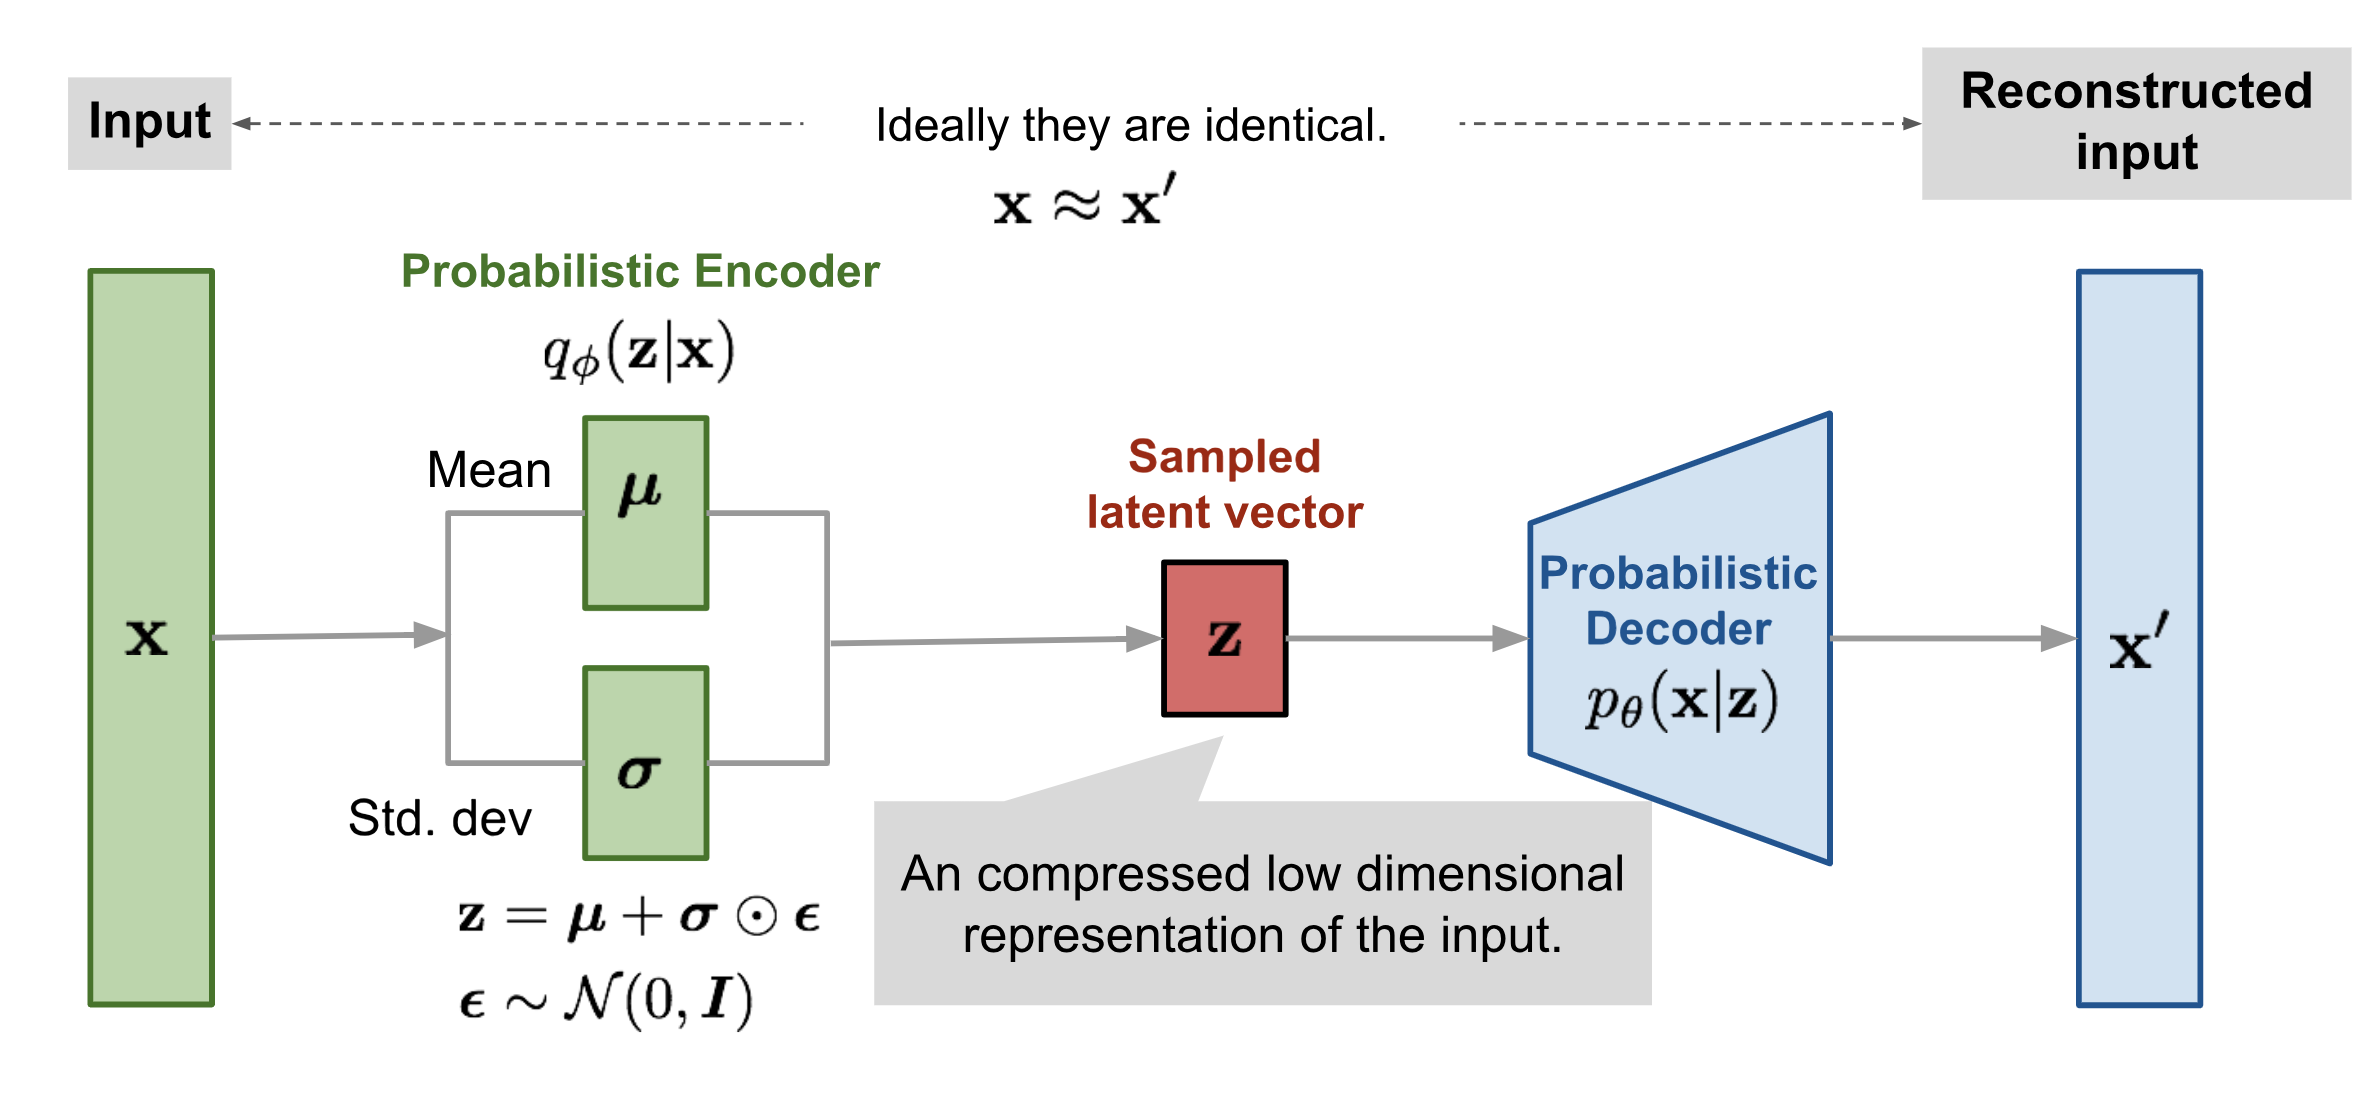
\includegraphics[width=\linewidth]{figs/vae-gaussian.png}
	\end{figure}
	\hrule\medskip
	{\scriptsize \href{https://lilianweng.github.io/lil-log/2018/08/12/from-autoencoder-to-beta-vae.html}{https://lilianweng.github.io/lil-log/2018/08/12/from-autoencoder-to-beta-vae.html}}
	
\end{frame}
%=======
\begin{frame}{VAE limitations}
	\begin{itemize}
		\item Poor variational posterior distribution (encoder)
		\[
		q(\bz | \bx, \bphi) = \mathcal{N}(\bz| \bmu_{\bphi}(\bx), \bsigma^2_{\bphi}(\bx)).
		\]
		\item Poor prior distribution
		\[
		p(\bz) = \mathcal{N}(0, \mathbf{I}).
		\]
		\item Poor probabilistic model (decoder)
		\[
		p(\bx | \bz) = \mathcal{N}(\bx| \bmu_{\btheta}(\bz), \bsigma^2_{\btheta}(\bz)).
		\]
		\item Loose lower bound
		\[
		p(\bx | \btheta) - \mathcal{L}(q, \btheta) = (?).
		\]
	\end{itemize}
\end{frame}
%=======
\begin{frame}{Variational posterior}
	
	We wish $KL(q(\bz | \bx, \bphi) || p(\bz | \bx, \btheta)) = 0$. \\
	(In this case the lower bound is tight $p(\bx | \btheta) = \mathcal{L}(q, \btheta)$). \\
	\vspace{0.5cm}
	Normal variational distribution $q(\bz | \bx, \bphi) = \mathcal{N}(\bz| \bmu_{\bphi}(\bx), \bsigma^2_{\bphi}(\bx))$ is poor (e.g. has only one mode). \\
	\vspace{0.5cm}
	Flows models transform simple base distribution to compex one using invertible transformation with simple Jacobian. \\
	\vspace{0.5cm}
	How to use flows in VAE?
\end{frame}
%=======
\begin{frame}{Flows in VAE}
	Apply the sequence of transformations to the random variables 
	\[
	\bz_0 \sim q_0(\bz | \bx, \bphi) = \mathcal{N}(\bz| \bmu_{\bphi}(\bx), \bsigma^2_{\bphi}(\bx)).
	\]
	Here, $q_0(\bz | \bx, \bphi)$ plays the role of a base distribution.
	\[
	\bz_0 \xrightarrow{g_1} \bz_1 \xrightarrow{g_2} \dots \xrightarrow{g_K} \bz_K.
	\]
	Each $g_k $ is a flow transformation (e.g. planar, radial, coupling layer).
	\[
	\log q_K(\bz_K) = \log q_0(\bz_0) - \sum_{k=1}^K \log \left| \det \left( \frac{\partial g_k(\bz_{k - 1})}{\partial \bz_{k-1}} \right) \right|.
	\]
	
	\vfill
	\hrule\medskip
	{\scriptsize \href{https://arxiv.org/pdf/1505.05770.pdf}{https://arxiv.org/pdf/1505.05770.pdf}} 
\end{frame}
%=======
\begin{frame}{Flows in VAE}
	\[
	\log q_K(\bz_K) = \log q_0(\bz_0) - \sum_{k=1}^K \log \left| \det \left( \frac{\partial g_k(\bz_{k - 1})}{\partial \bz_{k-1}} \right) \right|.
	\]
	Now the variational posterior is $q_K(\bz_K | \bx, \bphi)$.
	\begin{align*}
		\mathcal{L} (\bphi, \btheta)  &= \mathbb{E}_{q_K(\bz_K | \bx, \bphi)} \log \frac{p(\bx, \bz_K | \btheta)}{q_K(\bz_K| \bx, \phi)} \\
		&= \mathbb{E}_{q_K(\bz_K | \bx, \bphi)} \bigl[\log p(\bx, \bz_K | \btheta) - \log q_K(\bz_K| \bx, \phi) \bigr] \\
		&= \mathbb{E}_{q_0(\bz_0 | \bx, \bphi)} \bigl[\log p(\bx, \bz_K | \btheta) - \log q_K(\bz_K| \bx, \phi) \bigr] \\
		&= \mathbb{E}_{q_0(\bz_0 | \bx, \bphi)} \bigg[\log p(\bx, \bz_K | \btheta) -  \log q_0(\bz_0 | \bx, \bphi ) - \\ & - \sum_{k=1}^K \log \left| \det \left( \frac{\partial g_k(\bz_{k - 1})}{\partial \bz_{k-1}} \right) \right| \bigg].
	\end{align*}
	\vfill
	\hrule\medskip
	{\scriptsize \href{https://arxiv.org/pdf/1505.05770.pdf}{https://arxiv.org/pdf/1505.05770.pdf}} 
\end{frame}
%=======
\begin{frame}{Gaussian autoregressive model}
	Consider autoregressive model
	\[
		p(\bx | \btheta) = \prod_{i=1}^m p(x_i | \bx_{1:i - 1}, \btheta),
	\]
	with conditionals
	\[
	p(x_i | \bx_{1:i - 1}, \btheta) = \mathcal{N} \left(\hat{\mu}_i(\bx_{1:i-1}), \hat{\sigma}^2_i (\bx_{1:i-1})\right).
	\]
	\vspace{-0.5cm}
	\begin{block}{Sampling}
		\[
		x_i = \hat{\sigma}_i (\bx_{1:i-1}) \cdot z_i + \hat{\mu}_i(\bx_{1:i-1}), \quad z_i \sim \mathcal{N}(0, 1).
		\]
	\end{block}
	Sampling from autoregressive model is sequential. \\
	Note that we could interpret this sampling as a transormation $\bx = g(\bz, \btheta)$, where $\bz$ comes from base distribution $\mathcal{N}(0, 1)$.
\end{frame}
%=======
\begin{frame}{Gaussian autoregressive model}
	\begin{block}{Sampling}
		\vspace{-0.5cm}
		\[
		x_i = \hat{\sigma}_i (\bx_{1:i-1}) \cdot z_i + \hat{\mu}_i(\bx_{1:i-1}), \quad z_i \sim \mathcal{N}(0, 1).
		\]
		\vspace{-0.5cm}
	\end{block}
	\begin{block}{Jacobian}
		\vspace{-0.5cm}
		\[
		\log \left|\det \left( \frac{\partial f(\bx, \btheta)}{\partial \bx} \right) \right| = -\log \left|\det \left( \frac{\partial g(\bz, \btheta)}{\partial \bz} \right) \right| = - \sum_{i = 1}^m \log \hat{\sigma}_i (\bx_{1:i-1}).
		\]
		\vspace{-0.5cm}
	\end{block} 
	\begin{block}{Inverse transform}
		\vspace{-0.5cm}
		\[
		z_i = \left(x_i - \hat{\mu}_i(\bx_{1:i-1}) \right) \cdot \frac{1}{\hat{\sigma}_i (\bx_{1:i-1}) }.
		\]
	\end{block}
	We get an autoregressive model with tractable (triangular) Jacobian, which is easily invertible. It is a flow!
\end{frame}
%=======
\begin{frame}{Inverse autoregressive flow (IAF)}
	
	\begin{block}{Gaussian autoregressive model ($\bz \rightarrow \bx$)}
		\vspace{-0.2cm}
		\[
			x_i = \hat{\sigma}_i (\bx_{1:i-1}) \cdot z_i + \hat{\mu}_i(\bx_{1:i-1}).
		\]
		\[
			z_i = \left(x_i - \hat{\mu}_i(\bx_{1:i-1}) \right) \cdot \frac{1}{ \hat{\sigma}_i (\bx_{1:i-1})}.
		\]
		\vspace{-0.3cm}
	\end{block}
	This process is sequential. \\
	Let use the following reparametrization:
	$\hat{\bsigma} = \frac{1}{\bsigma}; \quad \hat{\bmu} = - \frac{\bmu}{\bsigma}.$
	
	\begin{block}{Inverse transform ($\bx \rightarrow \bz$)}
		\vspace{-0.2cm}
		\[
			z_i = \bsigma_i (\bx_{1:i-1}) \cdot x_i + \bmu_i(\bx_{1:i-1}).
		\]
		\[
			x_i = \left( z_i - \bmu_i(\bx_{1:i-1})\right) \cdot \frac{1}{\bsigma_i (\bx_{1:i-1}) }.
		\]
		\vspace{-0.3cm}
	\end{block}
	This process is \textbf{not} sequential.
	\vfill
	\hrule\medskip
	{\scriptsize \href{https://arxiv.org/pdf/1606.04934.pdf}{https://arxiv.org/pdf/1606.04934.pdf}} 
\end{frame}
%=======
\begin{frame}{Inverse autoregressive flow (IAF)}
	
	\begin{block}{Inverse transform ($\bx \rightarrow \bz$)}
		\vspace{-0.2cm}
		\[
			z_i = \bsigma_i (\bx_{1:i-1}) \cdot x_i + \bmu_i(\bx_{1:i-1}).
		\]
		\[
			x_i = \left( z_i - \bmu_i(\bx_{1:i-1})\right) \cdot \frac{1}{\bsigma_i (\bx_{1:i-1})}.
		\]
		\vspace{-0.3cm}
	\end{block}
	Inverse autoregressive flow use such inverted autoregressive model as a flow in VAE:
	\[
		\bz_0 = \bsigma_0(\bx) \cdot \bepsilon + \bmu_0(\bx), \quad \bepsilon \sim \mathcal{N}(0, 1); \quad (q_0(\bz_0 | \bx, \bphi))
	\]
	\[
		\bz_k = \bsigma_k(\bz_{k - 1}) \cdot \bz_{t-1} + \bmu_k(\bz_{k - 1}), \quad k \geq 1 \quad (q_k(\bz_k | \bx, \bphi)).
	\]
	\vfill
	\hrule\medskip
	{\scriptsize \href{https://arxiv.org/pdf/1606.04934.pdf}{https://arxiv.org/pdf/1606.04934.pdf}} 
\end{frame}
%=======
\begin{frame}{Flows}
\begin{figure}
	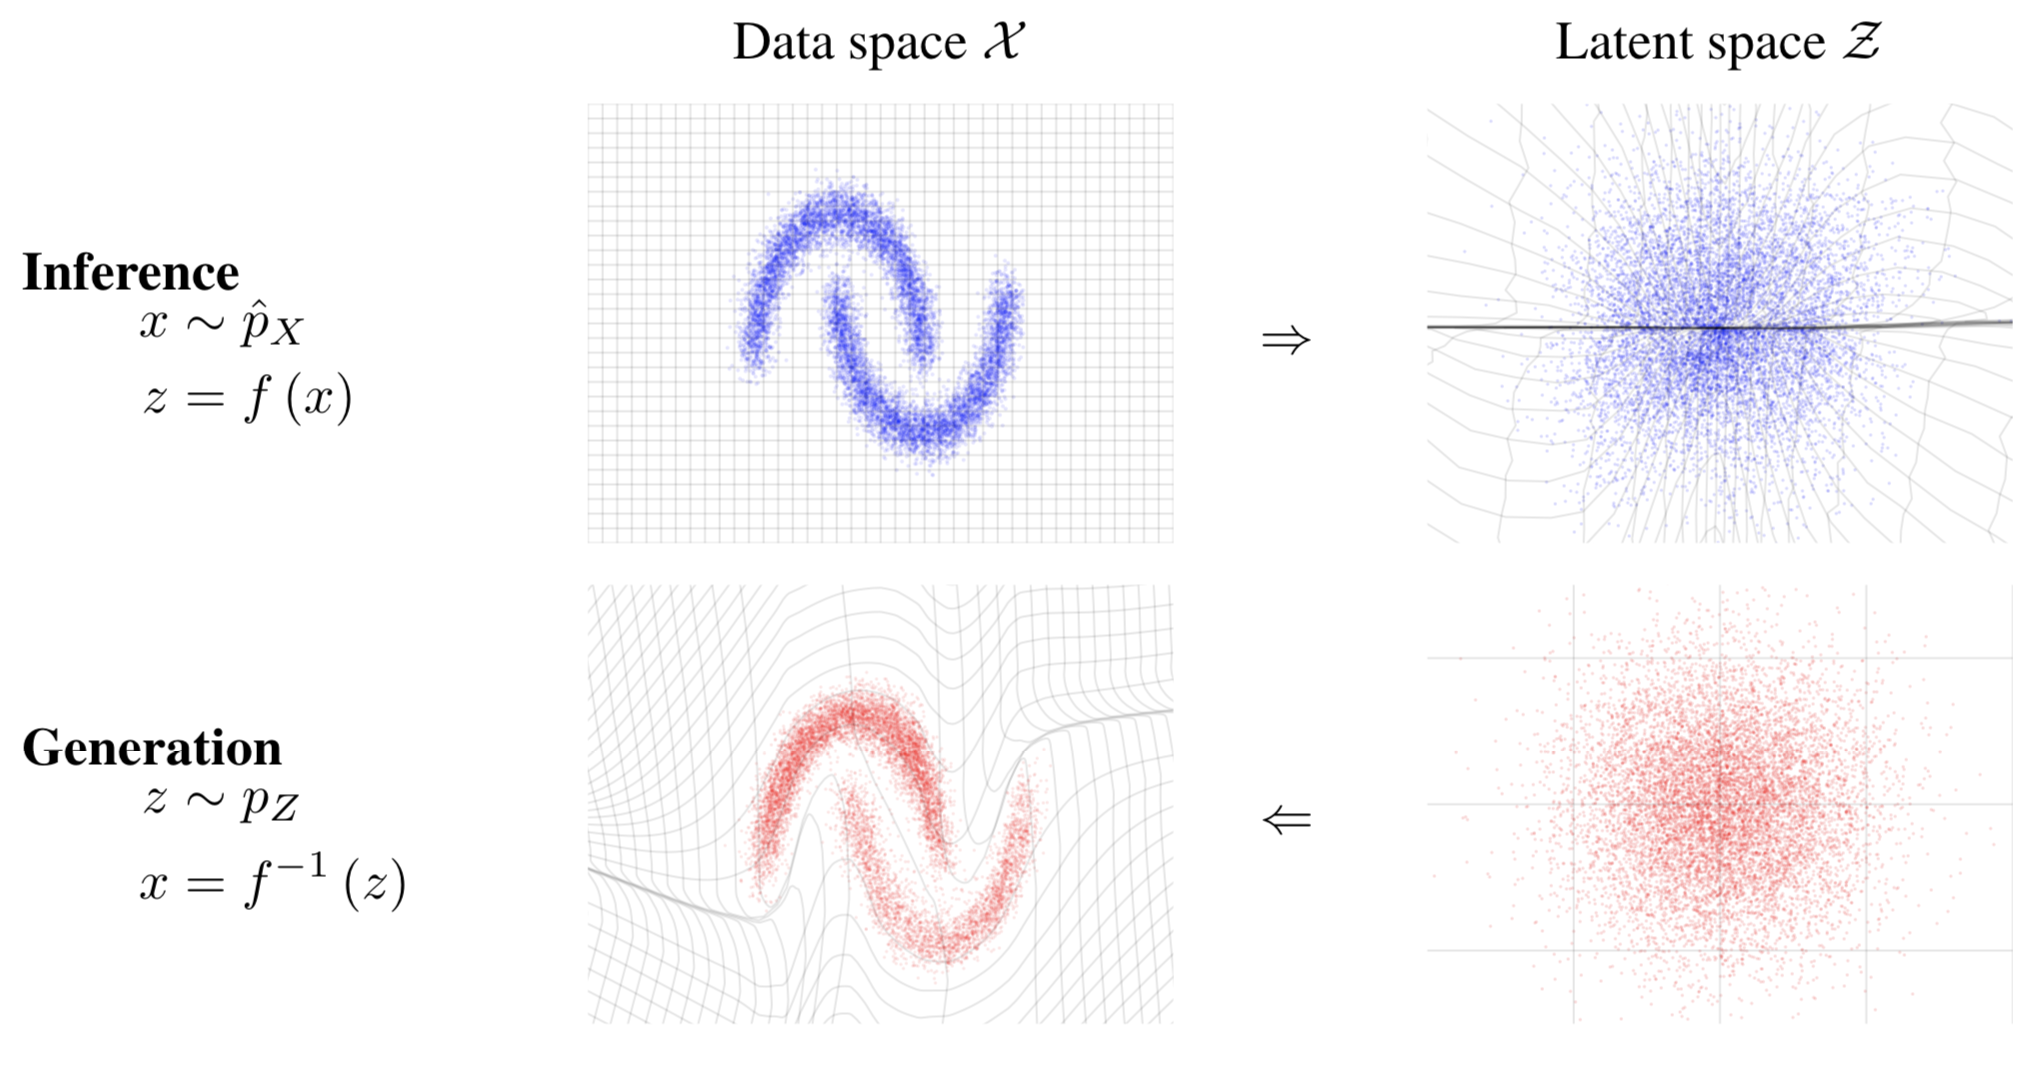
\includegraphics[width=0.8\linewidth]{figs/flows_how2.png}
\end{figure}
\begin{itemize}	
	\item Inference mode in autoregressive flows is used for density estimation task.
	\item Generation mode in autoregressive flows (IAF) is used for stochastic variational inference to get more flexible posterior distribution.
\end{itemize}
\vfill
\hrule\medskip
{\scriptsize \href{https://arxiv.org/pdf/1605.08803.pdf}{https://arxiv.org/pdf/1605.08803.pdf}} 
\end{frame}
%=======
\begin{frame}{Inverse autoregressive flow (IAF)}
	\begin{figure}
		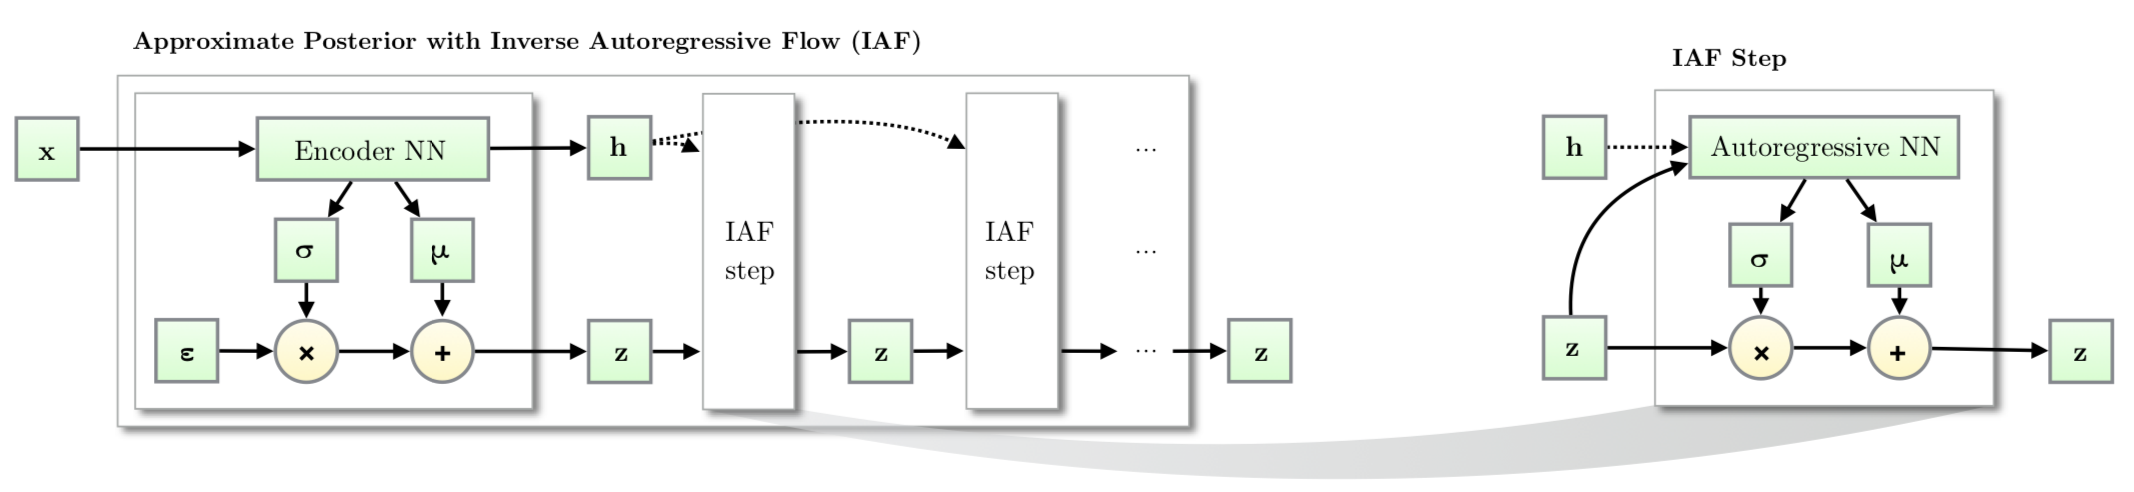
\includegraphics[width=\linewidth]{figs/iaf2.png}
	\end{figure}
	\begin{figure}
		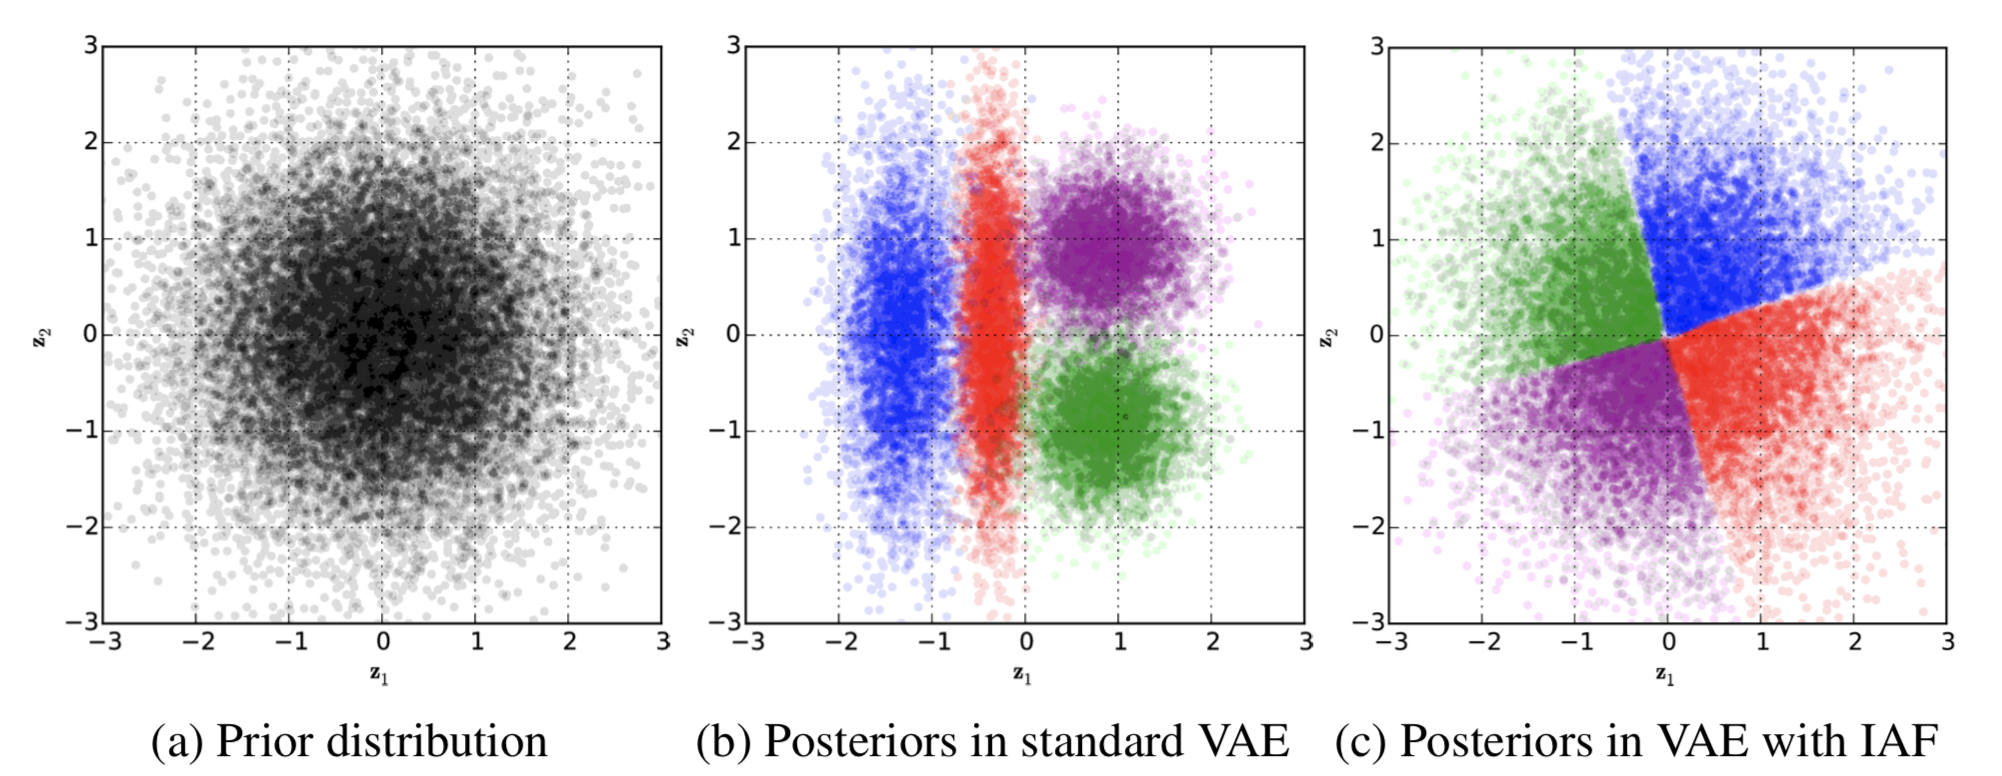
\includegraphics[width=\linewidth]{figs/iaf1.png}
	\end{figure}
	\vfill
	\hrule\medskip
	{\scriptsize \href{https://arxiv.org/pdf/1606.04934.pdf}{https://arxiv.org/pdf/1606.04934.pdf}} 
\end{frame}
%=======
\begin{frame}{Masked autoregressive flow (MAF)}
	\begin{block}{Gaussian autoregressive model}
	\vspace{-0.5cm}
	\[
		p(\bx | \btheta) = \prod_{i=1}^m p(x_i | \bx_{1:i - 1}, \btheta) = \prod_{i=1}^m \mathcal{N} \left(x_i | \mu_i(\bx_{1:i-1}), \sigma^2_i (\bx_{1:i-1})\right).
	\]
	\vspace{-0.5cm}
	\end{block}
	We could use MADE (masked autoencoder) as conditional model. The sampling order could be crucial.
	\begin{figure}
		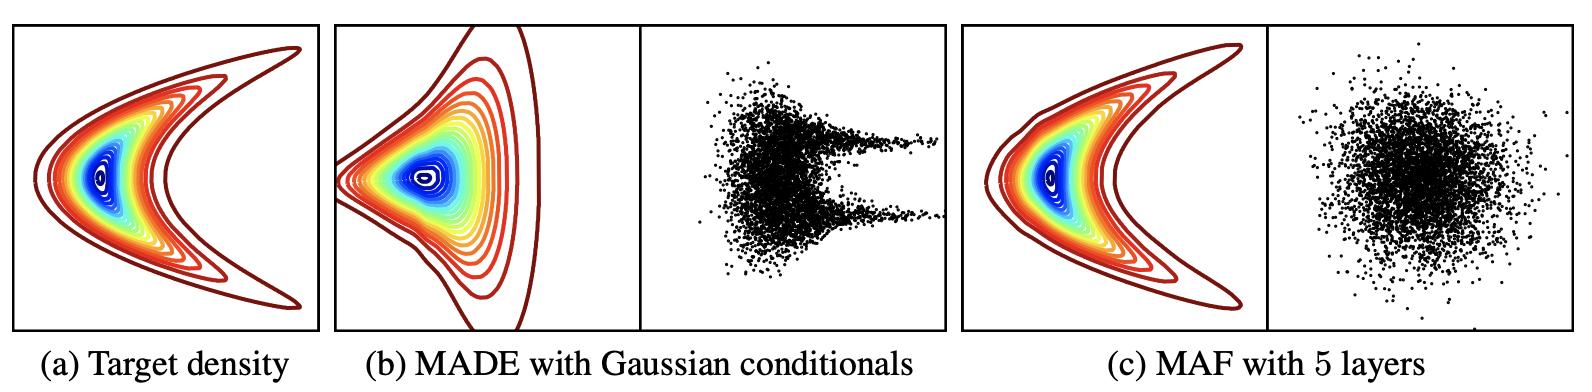
\includegraphics[width=\linewidth]{figs/maf1.png}
	\end{figure}
	Samples from the base distribution could be an indicator of how good the flow was fitted. \\
	\vfill
	\hrule\medskip
	{\scriptsize \href{https://arxiv.org/pdf/1705.07057.pdf}{https://arxiv.org/pdf/1705.07057.pdf}} 
\end{frame}
%=======
\begin{frame}{Masked autoregressive flow (MAF)}
	\begin{block}{Gaussian autoregressive model}
		\vspace{-0.5cm}
		\[
		p(\bx | \btheta) = \prod_{i=1}^m p(x_i | \bx_{1:i - 1}, \btheta) = \prod_{i=1}^m \mathcal{N} \left(x_i | \mu_i(\bx_{1:i-1}), \sigma^2_i (\bx_{1:i-1})\right).
		\]
		\vspace{-0.5cm}
	\end{block}
	\begin{figure}
		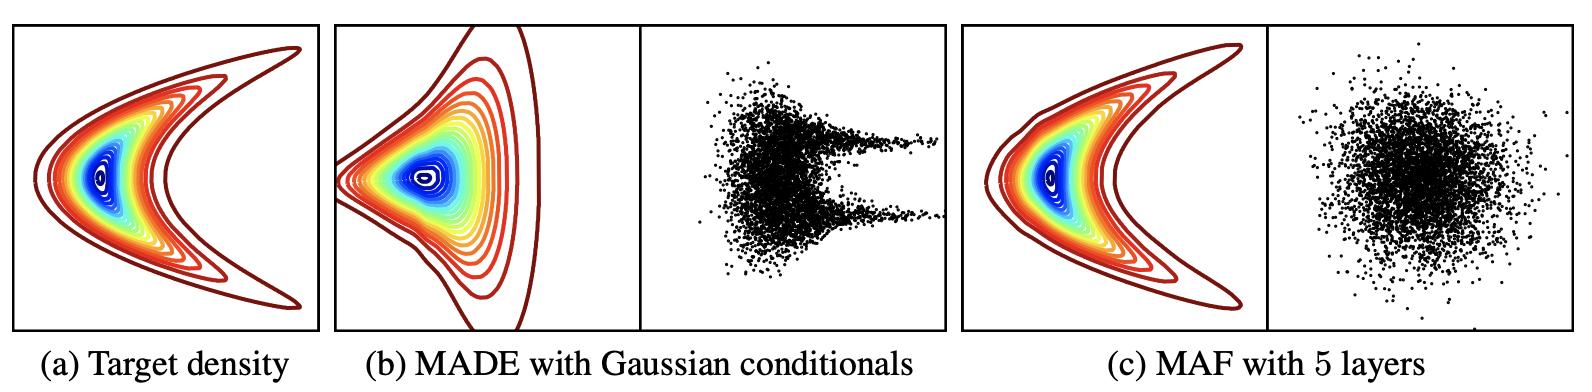
\includegraphics[width=\linewidth]{figs/maf1.png}
	\end{figure}
	MAF is just a stacked MADE model.
	\vfill
	\hrule\medskip
	{\scriptsize \href{https://arxiv.org/pdf/1705.07057.pdf}{https://arxiv.org/pdf/1705.07057.pdf}} 
\end{frame}
%=======
\begin{frame}{MAF vs IAF}
	\begin{block}{Sampling and inverse transform in MAF}
		\vspace{-0.2cm}
		\[
			x_i = \hat{\sigma}_i (\bx_{1:i-1}) \cdot z_i + \hat{\mu}_i(\bx_{1:i-1}).
		\]
		\[
			z_i = \left(x_i - \hat{\mu}_i(\bx_{1:i-1}) \right) \cdot \frac{1}{\hat{\sigma}_i (\bx_{1:i-1}) }.
		\]
		\vspace{-0.5cm}
		\begin{itemize}
			\item Sampling is slow (sequential).
			\item Density estimation is fast.
		\end{itemize}
	\end{block}
	\begin{block}{Sampling and inverse transform in IAF}
		\vspace{-0.2cm}
		\[
			z_i = \sigma_i (\bx_{1:i-1}) \cdot x_i + \mu_i(\bx_{1:i-1}).
		\]
		\[
			x_i = \left(z_i - \mu_i(\bx_{1:i-1}) \right) \cdot \frac{1}{\sigma_i (\bx_{1:i-1})}.
		\]
		\vspace{-0.3cm}
		\begin{itemize}
			\item Sampling is fast.
			\item Density estimation is slow (sequential).
		\end{itemize}
	\end{block}
	
	\vfill
	\hrule\medskip
	{\scriptsize \href{https://arxiv.org/pdf/1705.07057.pdf}{https://arxiv.org/pdf/1705.07057.pdf}} 
\end{frame}
%=======
\begin{frame}{MAF vs IAF}
	\small{
		\begin{block}{Theorem}
			Training a MAF with maximum likelihood corresponds to fitting an implicit IAF  with stochastic variational inference where the posterior is taken to be the base density:
			\[  
			\max_{\btheta} p(\bX | \btheta) \quad \Leftrightarrow \quad \min_{\btheta} KL\left(p(\bz | \btheta) || \pi(\bz)\right)
			\]
			(Here, $\pi(\bz)$ is a base distribution, $\pi(\bx)$ is a data distribution).
		\end{block}
		\begin{block}{Proof}
			\vspace{-0.5cm}
			\begin{multline*}
				KL\left(p(\bz | \btheta) || \pi(\bz) \right) = \mathbb{E}_{p(\bz | \btheta)} \bigl[ \log p(\bz | \btheta) - \log \pi(\bz) \bigr] = \\ 
				= \mathbb{E}_{p(\bz | \btheta)} \left[ \log \pi(g(\bz)) + \log \left| \det \left( \frac{\partial g(\bz)}{\partial \bz}\right) \right| - \log \pi(\bz) \right] = \\
				= \mathbb{E}_{\pi(\bx)} \left[ \log \pi(\bx) - \log \left| \det \left( \frac{\partial f(\bx)}{\partial \bx}\right) \right| - \log \pi(f(\bx)) \right].
			\end{multline*}
		\end{block}
	}
	\vfill
	\hrule\medskip
	{\scriptsize \href{https://arxiv.org/pdf/1705.07057.pdf}{https://arxiv.org/pdf/1705.07057.pdf}} 
\end{frame}
%=======
\begin{frame}{MAF vs IAF}
	\begin{block}{Proof (continued)}
		{\small
			\begin{multline*}
				KL\left(p(\bz | \btheta) || \pi(\bz) \right) = \mathbb{E}_{\pi(\bx)} \left[ \log \pi(\bx) - \log \left| \det \left( \frac{\partial f(\bx)}{\partial \bx}\right) \right| - \log \pi(f(\bx)) \right] = \\
				= \mathbb{E}_{\pi(\bx)} \bigl[ \log \pi(\bx) - \log p(\bx | \btheta) \bigr] = KL (\pi(\bx) || p(\bx | \btheta)).
			\end{multline*}
			\begin{align*}
				\argmin_{\btheta}  KL (\pi(\bx) || p(\bx | \btheta)) &= \argmin_{\btheta} \mathbb{E}_{\pi(\bx)} \left[ \log \pi(\bx) - \log p(\bx | \btheta) \right] \\
				&= \argmax_{\btheta} \mathbb{E}_{\pi(\bx)} \log p(\bx | \btheta)
			\end{align*}
			Unbiased estimator is MLE:
			\[
			\mathbb{E}_{\pi(\bx)} \log p(\bx | \btheta) = \sum_{i=1}^n \log p(\bx_i | \btheta).
			\]
		}
	\end{block}
	\vfill
	\hrule\medskip
	{\scriptsize \href{https://arxiv.org/pdf/1705.07057.pdf}{https://arxiv.org/pdf/1705.07057.pdf}} 
\end{frame}
%=======
\begin{frame}{MAF vs IAF vs RealNVP}
	\begin{block}{MAF}
		\vspace{-0.3cm}
		\[
		\bx = \hat{\bsigma} (\bx) \odot \bz + \hat{\bmu}(\bx).
		\]
		\vspace{-0.5cm}
		\begin{itemize}
			\item Calculating the density $p(\bx | \btheta)$ - 1 pass.
			\item Sampling - $m$ passes.
		\end{itemize}
	\end{block}
	\begin{block}{IAF}
		\vspace{-0.3cm}
		\[
		\bx = \bsigma (\bz) \odot \bz + \bmu(\bz).
		\]
		\vspace{-0.5cm}
		\begin{itemize}
			\item Calculating the density $p(\bx | \btheta)$ - $m$ passes.
			\item Sampling - 1 pass.
		\end{itemize}
	\end{block}
	\begin{block}{RealNVP}
		\vspace{-1cm}
		\begin{align*}
			\bx_{1:d} &= \bz_{1:d}; \\ \bx_{d:m} &= \bz_{d:m} \odot \exp \left(c_1(\bz_{1:d}, \btheta)\right) + c_2(\bx_{1:d}, \btheta).
		\end{align*}
		\vspace{-0.3cm}
	\end{block}
	
	\vfill
	\hrule\medskip
	{\scriptsize \href{https://arxiv.org/pdf/1705.07057.pdf}{https://arxiv.org/pdf/1705.07057.pdf}} 
\end{frame}
%=======
\begin{frame}{MAF vs IAF vs RealNVP}
	\begin{block}{RealNVP}
		\vspace{-0.7cm}
		\begin{align*}
			\bx_{1:d} &= \bz_{1:d}; \\ \bx_{d:m} &= \bz_{d:m} \odot \exp \left(c_1(\bz_{1:d}, \btheta)\right) + c_2(\bx_{1:d}, \btheta).
		\end{align*}
		\vspace{-0.8cm}
	\end{block}
	\begin{itemize}
		\item Calculating the density $p(\bx | \btheta)$ - 1 pass.
		\item Sampling - 1 pass.
	\end{itemize}

	RealNVP is a special case of MAF and IAF:
	\begin{block}{MAF}
		\vspace{-0.5cm}
		\begin{equation*}
			\begin{cases}
				\hat{\mu}_i  = \hat{\sigma}_i = 0, \, i = 1, \dots, d; \\
				\hat{\mu}_i, \hat{\sigma}_i \text{ -- functions of } \bx_{1:d}, \, i = d+1, \dots, m.
			\end{cases}
		\end{equation*}
		\vspace{-0.3cm}
	\end{block}
	\begin{block}{IAF}
		\vspace{-0.3cm}
		\begin{equation*}
			\begin{cases}
				\mu_i  = \sigma_i = 0, \, i = 1, \dots, d; \\
				\mu_i, \sigma_i \text{ -- functions of } \bz_{1:d}, \, i = d+1, \dots, m.
			\end{cases}
		\end{equation*}
	\end{block}
	\vfill
	\hrule\medskip
	{\scriptsize \href{https://arxiv.org/pdf/1705.07057.pdf}{https://arxiv.org/pdf/1705.07057.pdf}} 
\end{frame}
%=======
\begin{frame}{References}
	{\scriptsize
		\begin{itemize}
			
			\item \textbf{Glow:} Better Reversible Generative Models \\
			\href{https://arxiv.org/abs/1807.03039}{https://arxiv.org/abs/1807.03039} \\
			\textbf{Summary:} Extension of RealNVP. Suggests 1x1 reversible convolutions instead of reversing channel ordering. 1x1 conv is square matrix which could be easily be inversed. Compares 1x1 conv with reversing and fixed shuffling. 
			
			\item \textbf{Flow++:} Improving Flow-Based Generative Models with Variational Dequantization and Architecture Design \\
			\href{https://arxiv.org/abs/1902.00275}{https://arxiv.org/abs/1902.00275} \\
			\textbf{Summary:} Flow model which investigates the dequantization of discrete probability distribution. Derives ELBO objective with variational noise dequantization distribution. 
			
			\item \textbf{IAF}: Improving Variational Inference with Inverse Autoregressive Flow \\
			\href{https://arxiv.org/abs/1606.04934}{https://arxiv.org/abs/1606.04934} \\
			\textbf{Summary:} Introduce inverse autoregressive flow (IAF). Models each autoregressive conditional as gaussian with autoregressive means and covariances. Inverse transformation allows to parallelize sampling.
			
			\item \textbf{MAF}: Masked Autoregressive Flow for Density Estimation \\ 
			\href{https://arxiv.org/pdf/1705.07057.pdf}{https://arxiv.org/pdf/1705.07057.pdf} \\
			\textbf{Summary:} Similar to IAF. Give comprehensive overview with link to IAF and RealNVP.  MAF is suitable for density estimation, IAF as a recognition network.
		\end{itemize}
	}
\end{frame}
\end{document} 